%%%%%%%%%%%%%%%%%%%%%%%%%%%%%%%%%%%%%%%%%
% Beamer Presentation
% LaTeX Template
% Version 1.0 (10/11/12)
%
% This template has been downloaded from:
% http://www.LaTeXTemplates.com
%
% License:
% CC BY-NC-SA 3.0 (http://creativecommons.org/licenses/by-nc-sa/3.0/)
%
%%%%%%%%%%%%%%%%%%%%%%%%%%%%%%%%%%%%%%%%%

%----------------------------------------------------------------------------------------
%    PACKAGES AND THEMES
%----------------------------------------------------------------------------------------

\documentclass{beamer}

\usepackage[utf8]{inputenc}
\usepackage[T1]{fontenc}
\usepackage{graphicx}
\usepackage{listings}

\mode<presentation> {

% The Beamer class comes with a number of default slide themes
% which change the colors and layouts of slides. Below this is a list
% of all the themes, uncomment each in turn to see what they look like.

%\usetheme{default}
%\usetheme{AnnArbor}
%\usetheme{Antibes}
%\usetheme{Bergen}
%\usetheme{Berkeley}
%\usetheme{Berlin}
%\usetheme{Boadilla}
%\usetheme{CambridgeUS}
%\usetheme{Copenhagen}
%\usetheme{Darmstadt}
%\usetheme{Dresden}
%\usetheme{Frankfurt}
%\usetheme{Goettingen}
%\usetheme{Hannover}
%\usetheme{Ilmenau}
%\usetheme{JuanLesPins}
%\usetheme{Luebeck}
\usetheme{Madrid}
%\usetheme{Malmoe}
%\usetheme{Marburg}
%\usetheme{Montpellier}
%\usetheme{PaloAlto}
%\usetheme{Pittsburgh}
%\usetheme{Rochester}
%\usetheme{Singapore}
%\usetheme{Szeged}
%\usetheme{Warsaw}

% As well as themes, the Beamer class has a number of color themes
% for any slide theme. Uncomment each of these in turn to see how it
% changes the colors of your current slide theme.

%\usecolortheme{albatross}
%\usecolortheme{beaver}
%\usecolortheme{beetle}
%\usecolortheme{crane}
%\usecolortheme{dolphin}
%\usecolortheme{dove}
%\usecolortheme{fly}
%\usecolortheme{lily}
%\usecolortheme{orchid}
%\usecolortheme{rose}
%\usecolortheme{seagull}
\usecolortheme{seahorse}
%\usecolortheme{whale}
%\usecolortheme{wolverine}

%\setbeamertemplate{footline} % To remove the footer line in all slides uncomment this line
%\setbeamertemplate{footline}[page number] % To replace the footer line in all slides with a simple slide count uncomment this line

%\setbeamertemplate{navigation symbols}{} % To remove the navigation symbols from the bottom of all slides uncomment this line
}

\usepackage{graphicx} % Allows including images
\usepackage{booktabs} % Allows the use of \toprule, \midrule and \bottomrule in tables

%----------------------------------------------------------------------------------------
%    TITLE PAGE
%----------------------------------------------------------------------------------------

\title[Linux Container APIs]{Container management APIs} % The short title appears at the bottom of every slide, the full title is only on the title page

\author{Serge Hallyn} % Your name
\institute[Canonical] % Your institution as it will appear on the bottom of every slide, may be shorthand to save space
{
Canonical, Ltd \\ % Your institution for the title page
\medskip
\textit{serge.hallyn@ubuntu.com} % Your email address
}
\date{\today} % Date, can be changed to a custom date

\begin{document}

\lstset{language=sh}

\begin{frame}
\titlepage % Print the title page as the first slide
\end{frame}

\begin{frame}
\begin{figure}
  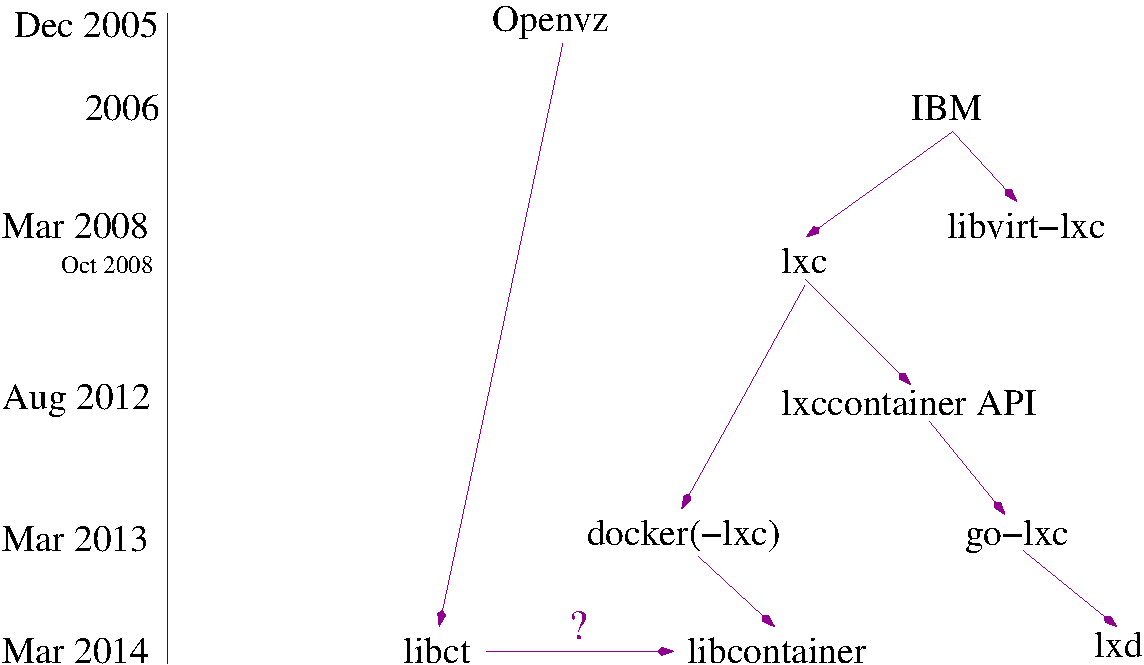
\includegraphics[width=\textwidth]{timeline.pdf}
\end{figure}
\end{frame}

\begin{frame}
\frametitle{Regular Usage: Overview}
\begin{itemize}
\item Let's first go over the basics:
  \begin{itemize}
  \item Download an image
  \item Run a command in a container
  \item Publish the new image
  \end{itemize}
\end{itemize}
\end{frame}

\begin{frame}[fragile]
\frametitle{Regular Usage: Docker}
\begin{itemize}
\item docker pull ubuntu
\item docker run -i -t ubuntu /usr/bin/touch cd
\item docker ps -a
{\tiny
\begin{verbatim}
ef45ea2cf7da        ubuntu:latest       "/usr/bin/touch cd"   10 seconds ago
d7bd5a48055f        ubuntu:latest       "/bin/bash"           19 hours ago
\end{verbatim}
}

\item docker run -i -it ubuntu /bin/ls
\item docker commit -m "add ab" f57b28609407 ubuntu:ab
{\tiny
\verb@f68322852844620ea3a0ee9fc86ae7f2016f344d031e80a5331fffaa8efcf61c@
}

\item sudo docker images
{\tiny
\begin{verbatim}
REPOSITORY          TAG                 IMAGE ID            CREATED             VIRTUAL SIZE
ubuntu              cd                  f68322852844        21 seconds ago      188.3 MB
ubuntu              latest              91e54dfb1179        4 weeks ago         188.3 MB
\end{verbatim}
}
\end{itemize}
\end{frame}

\begin{frame}
\frametitle{Regular Usage: LXD}
\begin{itemize}
\item lxc image list lxc:
\item lxc launch lxc:ubuntu/trusty/amd64 u1
\item lxc image list
\item lxc list
\item lxc exec u1 -- /usr/bin/touch/cd
\item lxc stop u1
\item lxc publish u1 myrepo:ubuntucd
\end{itemize}
\end{frame}

\begin{frame}
\frametitle{Regular Usage: LXC}
\begin{itemize}
\item lxc-create -t download -n w1 -- -d ubuntu -r wily -a amd64
\item lxc-ls -f
\item lxc-start -n u1
\item lxc-attach -n u1 -- touch /cd
\item lxc-stop -n u1
\item lxc-clone -s -o u1 -n u2
\item \texttt{Not image-based - no `publish' concept}
\end{itemize}
\end{frame}

\begin{frame}
\frametitle{Digging Deeper}
\begin{itemize}
\item Getting familiar with the commands is important
\item Docker and LXD have REST APIs
\item Go further building custom tools against library APIs
\end{itemize}
\end{frame}

\begin{frame}[fragile]
\frametitle{Docker REST API}
\begin{itemize}
\item List Images: \\
curl --unix-socket /run/docker.sock http:/images/json
\item Create a container: \\
\begin{lstlisting}
curl --unix-socket /run/docker.sock \
  -H "Content-Type: application/json" \
  -X POST http:/containers/create \
  -d '{ "Image": "ubuntu:latest", \
  "ExposedPorts":{"22/tcp":{}} , \
  "Binds": ["/home/ubuntu:/opt"], \
  "Entrypoint": "/sbin/init"}' \\
\end{lstlisting}
  \vspace{0.25in}
\textbf{ {"Id":"3b7e4b7aa...","Warnings":null} } \\

\item Start the container: \\
curl --unix-socket /run/docker.sock \
  -X POST http:/containers/ID/start \
  -d '{ "Binds":["/home/serge:/opt"] }'
\end{itemize}
\end{frame}

\begin{frame}
\begin{itemize}
\item curl --unix-socket /run/docker.sock -X GET http:/containers/json
\item curl --unix-socket /run/docker.sock -X POST http:/containers/ID/stop
\item curl --unix-socket /run/docker.sock -X DELETE  http:/containers/ID
\item curl --unix-socket /run/docker.sock -X DELETE  http:/containers/log
\item curl --unix-socket /run/docker.sock -X GET http:/containers/ID/logs?stdout=1
\end{itemize}
\end{frame}

\begin{frame}
\frametitle{Runc}
\begin{itemize}
\item A new way to run OpenContainers format containers
\item Requires
  \begin{itemize}
  \item untarred rootfs
  \item config.json: mounts (brief), user, env, capabilities, arch
  \item runtime.json: mounts(details), devices, security, hooks, more
  \end{itemize}
\end{itemize}
\end{frame}

\begin{frame}[fragile]
\frametitle{LXD REST API}
\begin{itemize}
\item List images: \\
{\tiny
  \begin{lstlisting}
curl --unix-socket /var/lib/lxd/unix.socket http:/1.0
  \end{lstlisting}
}

%\end{itemize}
%\end{frame}
%
%\begin{frame}[fragile]
%\begin{itemize}
%\item Create container: \\
%{\tiny
%  \begin{lstlisting}
%curl --unix-socket /var/lib/lxd/unix.socket http:/1.0/containers \
%  -X POST -d '{  "name":"x1", "source":{"type":"image","alias":"ubuntu" } }'
%  \end{lstlisting}
%}
%
%{\tiny
%\begin[verbatim}
%{"type":"async","status":"OK",
%"status_code":100,
%"operation":"/1.0/operations/e8b807a6-e19a-4cfe-ad69-2069ecaec14a",
%"resources":{"containers":["/1.0/containers/x1"]},
%"metadata":null}
%\end{verbatim}
%}

\item All documented at: \\
{\tiny
\url{https://github.com/lxc/lxd/blob/master/specs/rest-api.md}
}
\end{itemize}
\end{frame}

\begin{frame}[fragile]
\frametitle{Building new tools: lxd/lxc}
{\bf Create container in go:} \\
{\tiny
\begin{lstlisting}
func create(name, lxcpath string) error {
  c, err := lxc.NewContainer(name, lxcpath)
  if err != nil {
    return err
  }
  options := lxc.TemplateOptions{
    Template:             "download",
    Distro:               "ubuntu",
    Release:              "trusty",
    Arch:                 "amd64",
    FlushCache:           false,
    DisableGPGValidation: false,
  }
  err = c.Create(options)
  return err
\end{lstlisting}
}
\end{frame}

\begin{frame}[fragile]
\frametitle{Building new tools: lxd/lxc}
{\bf Get state of running container in python:} \\
{\tiny
\begin{lstlisting}
>>> import lxc
>>> c=lxc.Container("x1", "/var/run/lxd/containers")
>>> c.state
"RUNNING"
\end{lstlisting}
}
\end{frame}

\begin{frame}
\frametitle{Building new tools: libct}
\begin{itemize}
\item Libct is focused on creating container drivers
\item No concept of configuration files or image formats
\item Intended to be flexible
  \begin{itemize}
  \item Any combination of namespace sharing
  \item Any combination of security features
  \item Mount as you wish
  \item \dots you must do it all yourself
  \end{itemize}
\item Assume we create a container with lxc-start or docker,
\item Run "ps" in the container
\end{itemize}
\end{frame}

\begin{frame}[fragile]
\begin{figure}
{\tiny
  \begin{lstlisting}
/* Run a full system container as root */
int main(int argc, char **argv)
{
	libct_session_t s;
	ct_handler_t ct;
	ct_process_desc_t p;
	ct_process_t pr;
	struct ct_net_veth_arg va;
	ct_net_t nd, peernd;
	int ret;
	va.host_name = "hveth0";
	va.ct_name = "cveth0";

	printf("Setting up session\n");
	s = libct_session_open_local();
  printf("Creating in-memory container\n");
	ct = libct_container_create(s, "t1");
	p = libct_process_desc_create(s);
	if (libct_container_set_nsmask(ct,
   CLONE_NEWPID | CLONE_NEWNS | CLONE_NEWIPC |
 CLONE_NEWNET | CLONE_NEWUTS)) {
		printf("Unable to set nsmask\n");
		return -1;
	}

	printf("Setting up capabilities\n");
	/* fixme - get real caplist */
#define TEST_CAPS 0x1234
	libct_process_desc_set_caps(p, TEST_CAPS, CAPS_ALLCAPS);
  \end{lstlisting}
}
\end{figure}
\end{frame}

\begin{frame}[fragile]
\begin{figure}
{\tiny
  \begin{lstlisting}

	printf("Setting up network\n");
	nd = libct_net_add(ct, CT_NET_VETH, &va);
	if (libct_handle_is_err(nd)) {
		printf("Can't add hostnic\n");
		return -1;
	}
	peernd = libct_net_dev_get_peer(nd);
	if (libct_handle_is_err(peernd)) {
		printf("Can't get a veth peer\n");
		return -1;
	}


	if (libct_net_dev_set_master(peernd, "lxcbr0") < 0) {
		printf("Can't get set master\n");
		return -1;
	}

	printf("setting rootfs\n");
	if (libct_fs_set_root(ct, "/var/lib/lxc/t1/rootfs")) {
		printf("Unable to set root\n");
		return -1;
	}

	printf("adding filesystems\n");
	libct_fs_add_mount(ct, "proc", "/proc", 0, "proc", "");
	libct_fs_add_mount(ct, "sys", "/sys", 0, "sysfs", "");
  \end{lstlisting}
}
\end{figure}
\end{frame}

\begin{frame}[fragile]
\begin{figure}
{\tiny
  \begin{lstlisting}

	printf("setting up cgroups\n");
	if (libct_container_set_option(ct, LIBCT_OPT_CGROUP_SUBMOUNT, NULL) < 0) {
		printf("unable to set cgroup mounts option\n");
		return -1;
	}
	if (libct_controller_add(ct, CTL_DEVICES | CTL_FREEZER) < 0) {
		printf("unable to add cgroup controllers\n");
		return -1;
	}

	printf("setting up apparmor\n");
	libct_process_desc_set_lsm_label(p, "lxc-container-default");

	printf("Executing init\n");
	char *newargv[] = {"init", "--debug", NULL};
	pr = libct_container_spawn_execv(ct, p, "/sbin/init", newargv);
	if (libct_handle_is_err(pr)) {
		printf("Unable to start CT\n");
		return -1;
	}

	enum ct_state c = libct_container_state(ct);
	printf("current state is %d\n", (int)c);
	ret = libct_container_wait(ct);
	if (ret < 0) {
		printf("Unable to wait on the CT: %d\n", ret);
		return -1;
	}

	libct_container_destroy(ct);
	libct_session_close(s);

	printf("Container is alive\n");
	return 0;
}

  \end{lstlisting}
}
\end{figure}
\end{frame}

\begin{frame}
\frametitle{Building new tools: libcontainer}
\begin{itemize}
\item Written in go \\
only usable in go
\item runc implemented using libcontainer
\item Re-exec's self for container init
\end{itemize}
\end{frame}

\begin{frame}[fragile]
\begin{figure}
{\tiny
  \begin{lstlisting}
package main

import (
	"fmt"
	"os"
	"runtime"

	"github.com/opencontainers/runc/libcontainer"
	"github.com/opencontainers/runc/libcontainer/configs"
)

func init() {
	if len(os.Args) > 1 && os.Args[1] == "init" {
		runtime.GOMAXPROCS(1)
		runtime.LockOSThread()
		factory, _ := libcontainer.New("")
		if err := factory.StartInitialization(); err != nil {
			fmt.Printf("Failed init: %v\n", err)
			os.Exit(1)
		}
		fmt.Printf("Failed init: it returned\n")
		os.Exit(1)
	}
}
   \end{lstlisting}
}
\end{figure}
\end{frame}

\begin{frame}[fragile]
\begin{figure}
{\tiny
   \begin{lstlisting}
func main() {
	config := &configs.Config{
	    Rootfs: "/home/ubuntu/runc/rootfs",
	    Capabilities: []string{CAP_SYS_ADMIN}
	    Namespaces: configs.Namespaces([]configs.Namespace{
		{Type: configs.NEWNS},
		{Type: configs.NEWUTS},
		{Type: configs.NEWIPC},
		{Type: configs.NEWPID},
		{Type: configs.NEWNET},
	    }),
	    Mounts: []*configs.Mount{
	        {
		   Source: "proc",
		   Destination: "/proc",
		   Device: "proc",
		},
	    },
	    Cgroups: &configs.Cgroup{
		Name:            "test-container",
		Parent:          "system",
		AllowAllDevices: false,
		AllowedDevices:  configs.DefaultAllowedDevices,
	    },

	    Devices:  configs.DefaultAutoCreatedDevices,
	    Hostname: "testing",
	    Networks: []*configs.Network{
		{
		    Type:    "loopback",
		    Address: "127.0.0.1/0",
		    Gateway: "localhost",
		},
	    },
	}
}
   \end{lstlisting}
}
\end{figure}
\end{frame}

\begin{frame}[fragile]
\begin{figure}
{\tiny
   \begin{lstlisting}

	factory, err := libcontainer.New("/home/ubuntu/runc", libcontainer.InitArgs(os.Args[0], "init"))
	if err != nil {
		fmt.Printf("loading libcontainer factory failed: %s\n", err)
		os.Exit(1)
	}
	container, err := factory.Create("serue", config)
	if err != nil {
		fmt.Printf("factory.Load failed: %s\n", err)
		os.Exit(1)
	}

	process := &libcontainer.Process{
		Args: []string{"/bin/bash"},
		Env: []string{"PATH=/bin:/usr/bin:/sbin:/usr/sbin"},
		User: "0:0",
		Cwd: "/",
		Stdin: os.Stdin,
		Stdout: os.Stdout,
		Stderr: os.Stderr,
	}
	if err := container.Start(process); err != nil {
		os.Exit(1)
	}
	status, err := process.Wait()
	if err != nil {
		fmt.Printf("Error waiting: %s (status %v)\n", err, status)
		os.Exit(1)
	}
	fmt.Printf("At end: status is %v\n", status)
	container.Destroy()
}
  \end{lstlisting}
}
\end{figure}
\end{frame}

%------------------------------------------------

\end{document} 
